% =====================================================================
%  TP RCSF -- Clustering LEACH sous NS3 -- Rapport (4 pages)
%  Compilation :  tectonic rapport.tex     (ou xelatex rapport.tex, deux passes)
%  Les figures sont lues dans ../figures/ et resume.txt est inclus tel quel (annexe).
% =====================================================================
\documentclass[11pt,a4paper]{article}

\usepackage{fontspec}
\usepackage[french]{babel}
\setmainfont{texgyretermes}[Extension=.otf,UprightFont=*-regular,BoldFont=*-bold,
  ItalicFont=*-italic,BoldItalicFont=*-bolditalic]
\setsansfont{texgyreheros}[Extension=.otf,UprightFont=*-regular,BoldFont=*-bold,
  ItalicFont=*-italic,BoldItalicFont=*-bolditalic]
\setmonofont{lmmono10-regular}[Extension=.otf,ItalicFont=lmmono10-italic,BoldFont=lmmonolt10-bold]
\usepackage{amsmath}
\makeatletter\renewcommand\normalsize{\@setfontsize\normalsize{10.5}{12.3}}\makeatother
\renewcommand\small{\fontsize{9.5}{11}\selectfont}
\usepackage{microtype}
\usepackage[a4paper,top=1.6cm,bottom=1.8cm,left=1.7cm,right=1.7cm]{geometry}
\usepackage{graphicx,float,caption,subcaption,array,fancyvrb,enumitem}
\usepackage[hidelinks,pdftitle={TP RCSF -- Clustering LEACH sous NS3},
  pdfauthor={KOURA Lémiyi Stéphane Ulrich}]{hyperref}

\graphicspath{{../figures/}}
\setlength{\parskip}{0pt}\setlength{\emergencystretch}{2em}
\setlength{\parindent}{1.2em}
\renewcommand{\arraystretch}{1.12}
\captionsetup{font=small,labelfont=bf,skip=3pt}
\captionsetup[subfigure]{font=footnotesize,skip=2pt}
\setlist{itemsep=1pt,topsep=2pt,parsep=0pt}
\setlength{\textfloatsep}{6pt}
\setlength{\intextsep}{6pt}
\setcounter{topnumber}{3}\renewcommand{\topfraction}{0.9}\renewcommand{\bottomfraction}{0.9}\renewcommand{\textfraction}{0.08}\renewcommand{\floatpagefraction}{0.75}

\newcommand{\pct}{\,\%}
\newcommand{\pmv}[2]{#1\,$\pm$\,#2}
\newcommand{\code}[1]{\texttt{\detokenize{#1}}}
\newcommand{\nCH}{n_{\mathrm{CH}}}

\pagestyle{plain}

\begin{document}

% ---------------------------------------------------------------------
\begin{center}
{\LARGE\bfseries Clustering dans les RCSF : simulation de LEACH sous NS3}\\[5pt]
{\large Rapport de TP -- Réseaux sans fil}\\[3pt]
KOURA Lémiyi Stéphane Ulrich (SIE) \textperiodcentered{} M1 IBAM / UJKZ \textperiodcentered{} Octobre 2026
\end{center}
\vspace{-2pt}\hrule\vspace{4pt}

% =====================================================================
\section{Introduction}
Dans un réseau de capteurs sans fil (RCSF), la batterie n'est pas remplaçable : la durée de vie dépend donc de la répartition des transmissions,
dont le coût croît en $d^2$ puis en $d^4$ avec la distance. Le clustering réduit ce coût : les membres d'un cluster envoient leurs données à un chef de cluster
(CH) qui les agrège et les transmet à la station de base (BS). \textbf{LEACH} (Heinzelman \textit{et al.} [1,2]) élit les CH de façon probabiliste : au round $r$, un nœud qui n'a pas encore été CH dans l'époque
courante ($1/p$ rounds) le devient s'il tire un nombre inférieur au seuil
\[ T(n)=\frac{p}{1-p\,(r \bmod 1/p)} . \]
Un round comprend une phase d'initialisation (annonce ADV des CH, adhésion JOIN des membres au CH le plus proche, planning TDMA SCHEDULE) puis un régime permanent
(membres $\to$ CH, agrégation, CH $\to$ BS).

L'objectif du TP est de vérifier par simulation les affirmations du tableau comparatif du cours (consommation d'énergie, durée de vie, passage à l'échelle) et de montrer que LEACH est
\og un piège \fg{} : son élection ignore l'énergie résiduelle et la distance à la BS.

\textbf{Choix de modélisation.} Nous utilisons NS3 3.40 (modules \textit{core}, \textit{network} et \textit{mobility}), installé dans une VM Ubuntu 22.04 ARM64 (Vagrant + QEMU) sur Mac Apple Silicon.
NS3 fournit les nœuds, leurs positions, le temps simulé et le générateur aléatoire ; l'énergie suit exactement le modèle de premier ordre imposé, codé dans \code{leach.cc}
(444 lignes : \code{ElectCH}, \code{FormClusters}, \code{SteadyState}, \code{Record}). Le canal est idéal, avec une option de pertes aléatoires. Cet « niveau applicatif » donne la maîtrise totale des
valeurs imposées et une simulation rapide, mais ne modélise ni collisions ni interférences (voir §\ref{sec:ns3}).

% =====================================================================
\section{Configuration et validation}
\begin{table}[H]
\centering\small
\begin{tabular}{|l|l|l|l|}
\hline
\textbf{Paramètre} & \textbf{Valeur} & \textbf{Paramètre} & \textbf{Valeur}\\ \hline
Nœuds $N$ & 100 (50 et 300 pour l'échelle) & Zone & $200\times200$ m, positions aléatoires fixes\\
Station de base & $(100\,;\,250)$, hors de la zone & Énergie initiale & 0,5 J par nœud (50 J au total)\\
Rounds & 1000 (1 round = 1 s simulée) & Graines & 5 (\code{RngRun} 1 à 5, \code{SetSeed} 12345)\\
$E_{\mathrm{elec}}$ ; $\varepsilon_{\mathrm{fs}}$ & 50 nJ/bit ; 10 pJ/bit/m$^2$ & $\varepsilon_{\mathrm{mp}}$ ; $d_0$ & 0,0013 \textbf{pJ}/bit/m$^4$ ; 87,7 m\\
$E_{\mathrm{DA}}$ & 5 nJ/bit/signal & Paquets données / contrôle & 4000 bits / 200 bits\\
$p$ & 0,05 (époque de 20 rounds) & Débit radio ; portée ADV & 250 kbit/s ; 100 m\\
Repli si aucun CH & envoi direct à la BS & Pertes aléatoires & 0\pct{} (variante : 2\pct)\\ \hline
\end{tabular}
\caption{Paramètres de la simulation (imposés : $N$, zone, BS, énergie, rounds, modèle radio ; les autres sont des choix).}\label{tab:param}
\end{table}

Le modèle d'énergie est le modèle radio de premier ordre : pour émettre $k$ bits sur une distance $d$,
\[ E_{Tx}(k,d)=\begin{cases} E_{\mathrm{elec}}\,k+\varepsilon_{\mathrm{fs}}\,k\,d^2 & \text{si } d<d_0,\\[2pt] E_{\mathrm{elec}}\,k+\varepsilon_{\mathrm{mp}}\,k\,d^4 & \text{si } d\ge d_0,\end{cases}
\qquad E_{Rx}(k)=E_{\mathrm{elec}}\,k,\qquad d_0=\sqrt{\varepsilon_{\mathrm{fs}}/\varepsilon_{\mathrm{mp}}} . \]

\textbf{Unité de $\varepsilon_{\mathrm{mp}}$.} L'énoncé donne 0,0013 nJ/bit/m$^4$. Avec cette valeur, $d_0=\sqrt{10\,\mathrm{pJ}/1{,}3\,\mathrm{nJ}}\approx2{,}8$ m et presque toutes les liaisons seraient en $d^4$,
avec un coût 1000 fois trop élevé. Nous retenons donc 0,0013 \textbf{pJ}/bit/m$^4$ (valeur de la littérature LEACH, $d_0=87{,}7$ m, cohérent avec une zone de 200 m) ; ce choix reste à confirmer par l'enseignant.

\textbf{Validation.}
\begin{enumerate}[label=(\roman*)]
\item Calculs à la main (paquet de 4000 bits), recoupés par script : membre $\to$ CH à 30 m = 236 µJ ; CH $\to$ BS à 150 m = 2,83 mJ, à 200 m = 8,52 mJ, à 270 m = 27,8 mJ
(118 fois le coût membre $\to$ CH) ; réception d'un paquet = 200 µJ.
\item Round 0 (1 CH, 99 membres) : 89,6 mJ consommés, dont $\approx42$ mJ indépendants de la distance (émission 19,8 + réception 19,8 + agrégation 2,0 mJ) ; le reste est l'amplification et le contrôle.
\item Une réimplémentation Python indépendante (\code{ref_leach.py}, 10 graines) donne FND $\approx206$ et HND $\approx526$, contre 191 et 519 sous NS3 (écarts relatifs de 7\pct{} et 1\pct), très en dessous du facteur 2 qui révélerait une erreur.
\item Contrôle des 20 CSV : 1000 lignes, aucune valeur manquante, énergie totale non croissante.
\end{enumerate}

% =====================================================================
\section{Résultats}
Toutes les valeurs sont des moyennes sur \textbf{5 graines} $\pm$ écart-type (bandes ombrées des figures) ; 1 round = 1 s simulée.

\subsection{Expérience A : énergie et durée de vie ($N=100$)}
\begin{figure}[htbp]
\centering
\begin{subfigure}{0.465\textwidth}\centering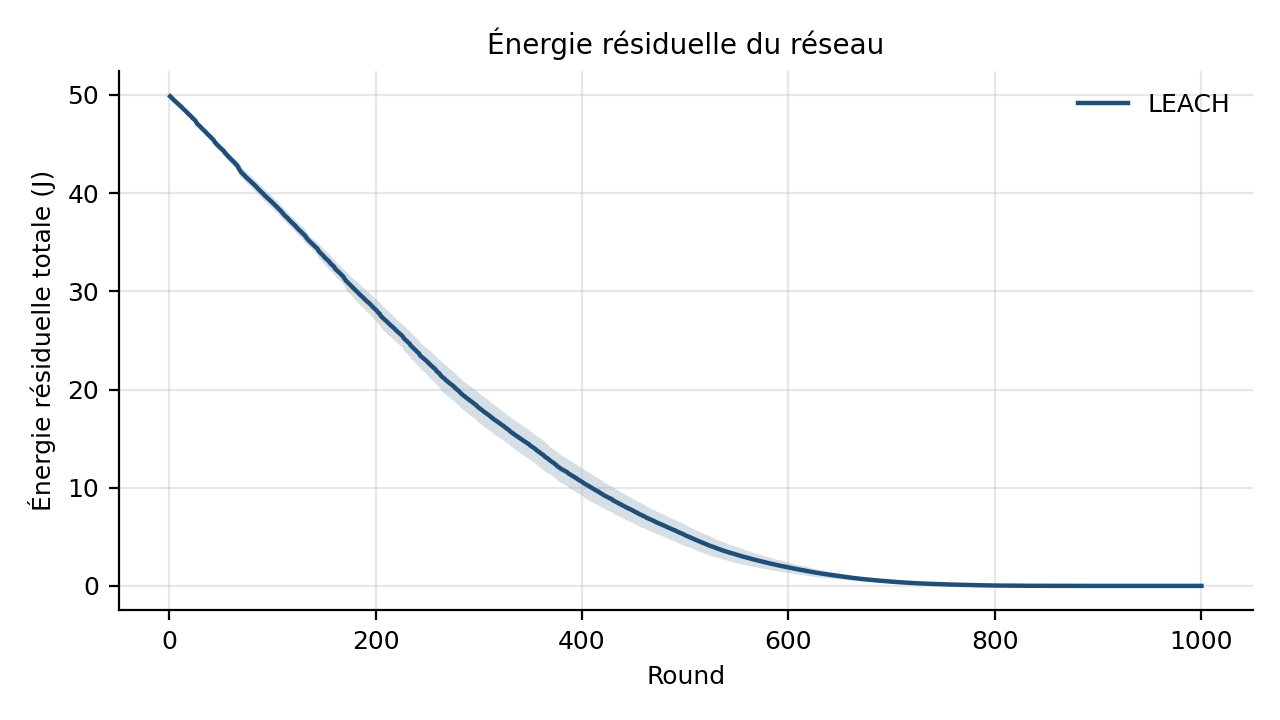
\includegraphics[width=\linewidth]{energie.png}\caption{Énergie résiduelle totale (J)}\label{fig:energie}\end{subfigure}\hfill
\begin{subfigure}{0.465\textwidth}\centering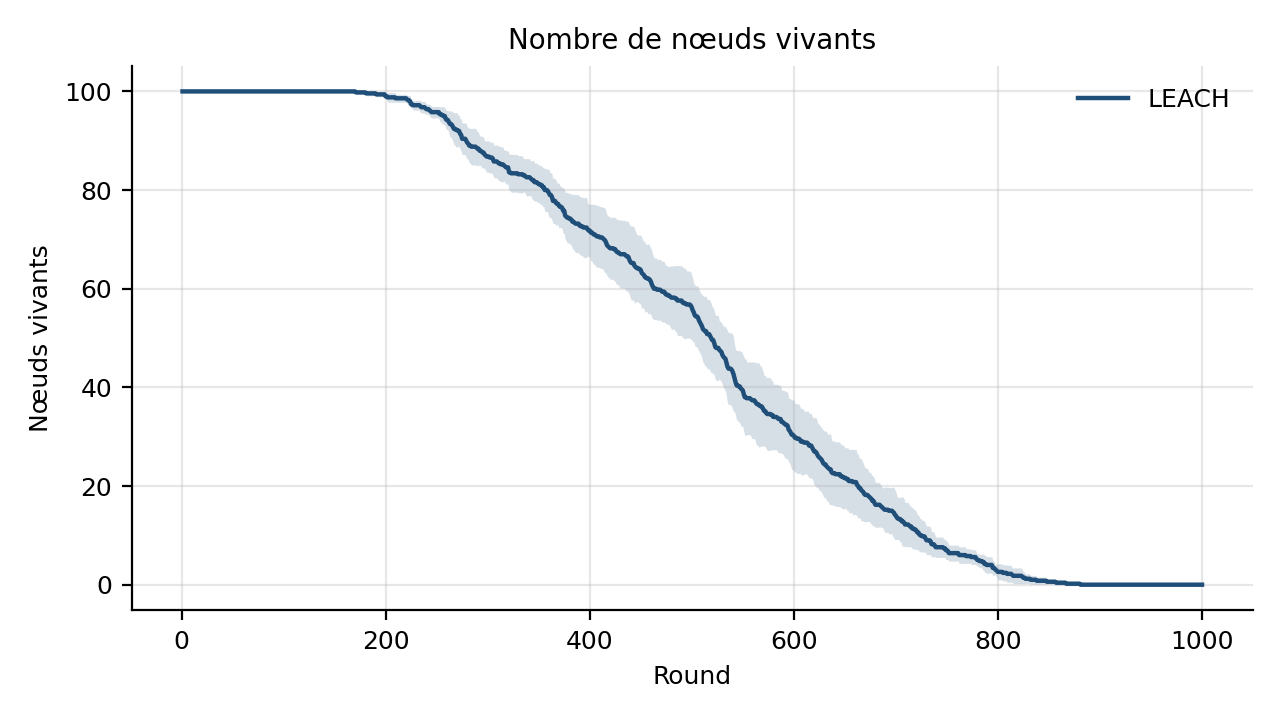
\includegraphics[width=\linewidth]{vivants.png}\caption{Nombre de nœuds vivants}\label{fig:vivants}\end{subfigure}
\caption{Expérience A : énergie du réseau et nœuds vivants en fonction du round ($N=100$, 5 graines).}\label{fig:A1}
\end{figure}



Les valeurs par graine figurent en annexe ; en moyenne FND $=191\pm14$, HND $=519\pm29$ et LND $=844\pm31$ rounds. L'énergie baisse presque linéairement au début ($\approx108$ mJ par round, soit 0,22\pct{} de l'énergie initiale) puis ralentit quand les nœuds meurent ($\approx54$ mJ par round entre les rounds 400 et 500) ;
elle est quasi nulle dès le round $\approx800$. Le premier nœud meurt au round \textbf{\pmv{191}{14}} alors qu'il reste \textbf{\pmv{58}{4}\pct} de l'énergie du réseau : l'énergie est mal répartie, non épuisée.
La période stable (FND/LND) ne représente que 23\pct{} de la durée de vie ; au HND il ne reste que 8\pct{} de l'énergie.

\begin{figure}[htbp]
\centering
\begin{subfigure}{0.465\textwidth}\centering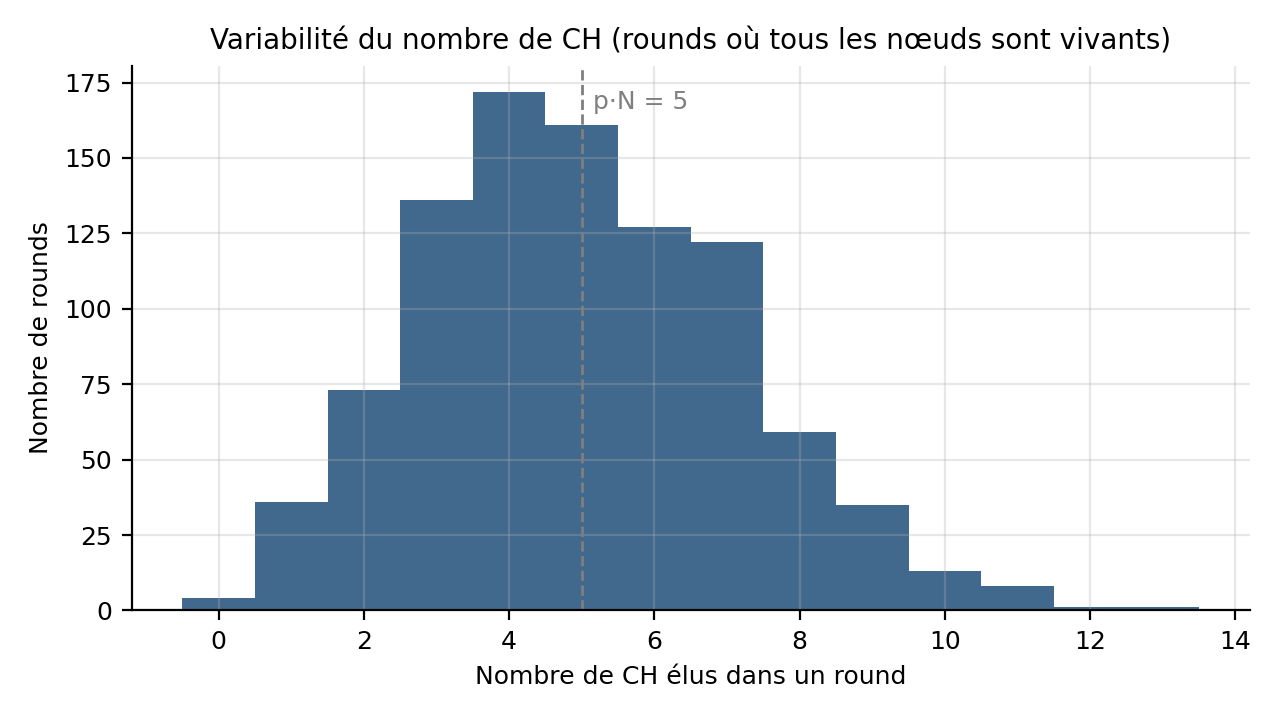
\includegraphics[width=\linewidth]{nch_histogramme.png}\caption{Nombre de CH par round}\label{fig:nch}\end{subfigure}\hfill
\begin{subfigure}{0.465\textwidth}\centering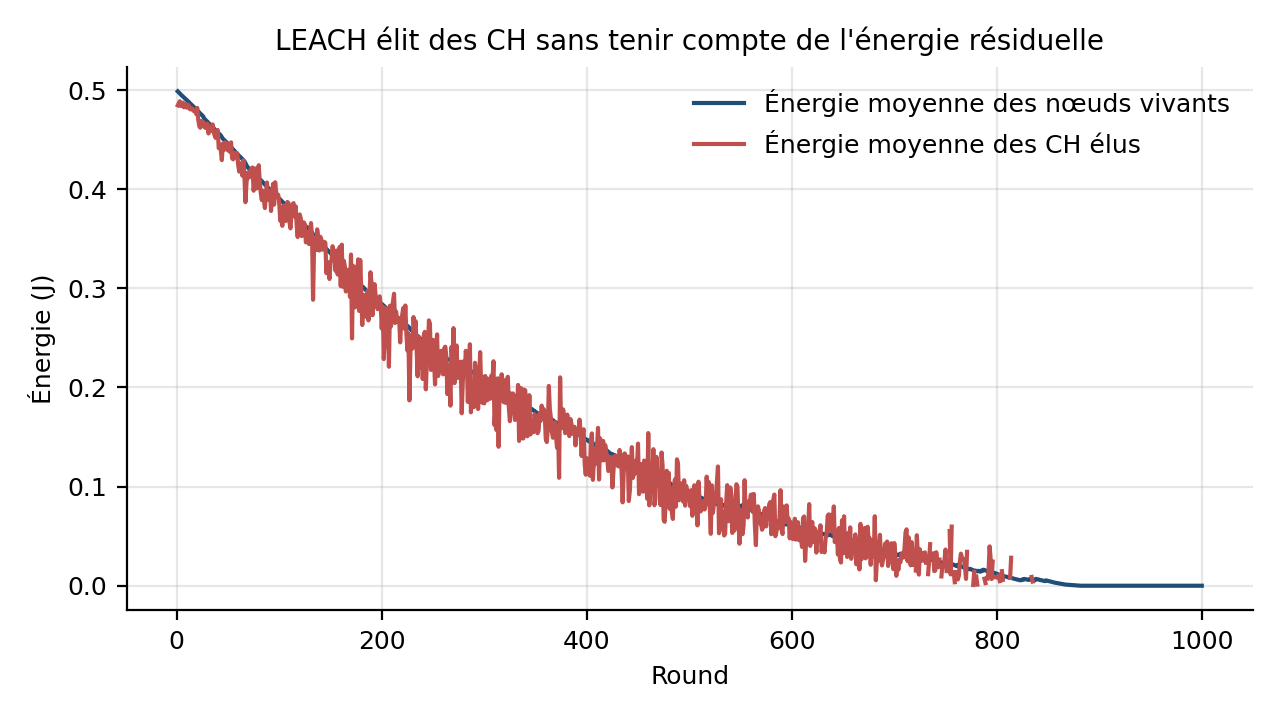
\includegraphics[width=\linewidth]{energie_ch_vs_moyenne.png}\caption{Énergie des CH élus et moyenne des vivants (J)}\label{fig:chmoy}\end{subfigure}
\caption{Variabilité du nombre de CH et énergie des CH élus ($N=100$, 5 graines).}\label{fig:A2}
\end{figure}

Le nombre de CH par round vaut 4,99 en moyenne (écart-type 2,17 ; de 0 à 13) : 23 rounds sur 948 en ont 10 ou plus et 4 n'en ont aucun, d'où le repli coûteux vers la BS (figure~\ref{fig:nch}).
Les deux courbes de la figure~\ref{fig:chmoy} se confondent (rapport énergie des CH / énergie moyenne $=0{,}96$, mesuré après les dépenses du round donc légèrement sous-estimé) : LEACH n'élit pas de préférence les nœuds riches.
Sur la réimplémentation Python (10 graines), la distance à la BS explique l'ordre de mort (corrélation de Spearman $-0{,}94$) : les 10 premiers nœuds morts sont à 243 m de la BS en moyenne, contre 160 m pour l'ensemble des nœuds.
Ces deux derniers chiffres ne viennent pas de NS3, dont les CSV ne contiennent pas de données par nœud.

\subsection{Expérience B : passage à l'échelle ($N=50,\,100,\,300$)}
\noindent\begin{minipage}[c]{0.605\textwidth}
\centering\footnotesize\setlength{\tabcolsep}{3.2pt}
\begin{tabular}{|c|c|c|c|c|c|c|}
\hline
$N$ & CH/round & Msg/round & Setup (ms) & FND & HND & LND\\ \hline
50 & 2,6 & 48,2 & 26,0 & \pmv{99}{16} & \pmv{302}{21} & \pmv{797}{55}\\
100 & 5,0 & 104,3 & 38,3 & \pmv{191}{14} & \pmv{519}{29} & \pmv{844}{31}\\
300 & 14,9 & 314,9 & 61,0 & \pmv{271}{14} & \pmv{638}{16} & 992$^{*}$\\ \hline
\end{tabular}
\captionof{table}{Passage à l'échelle. CH, messages et setup : moyennes sur les 30 premiers rounds ; FND/HND/LND en rounds. $^{*}$\,LND atteint dans 2 graines sur 5 ; dans les 3 autres, 1 nœud survit au round 1000.}\label{tab:echelle}
\end{minipage}\hfill
\begin{minipage}[c]{0.375\textwidth}
\centering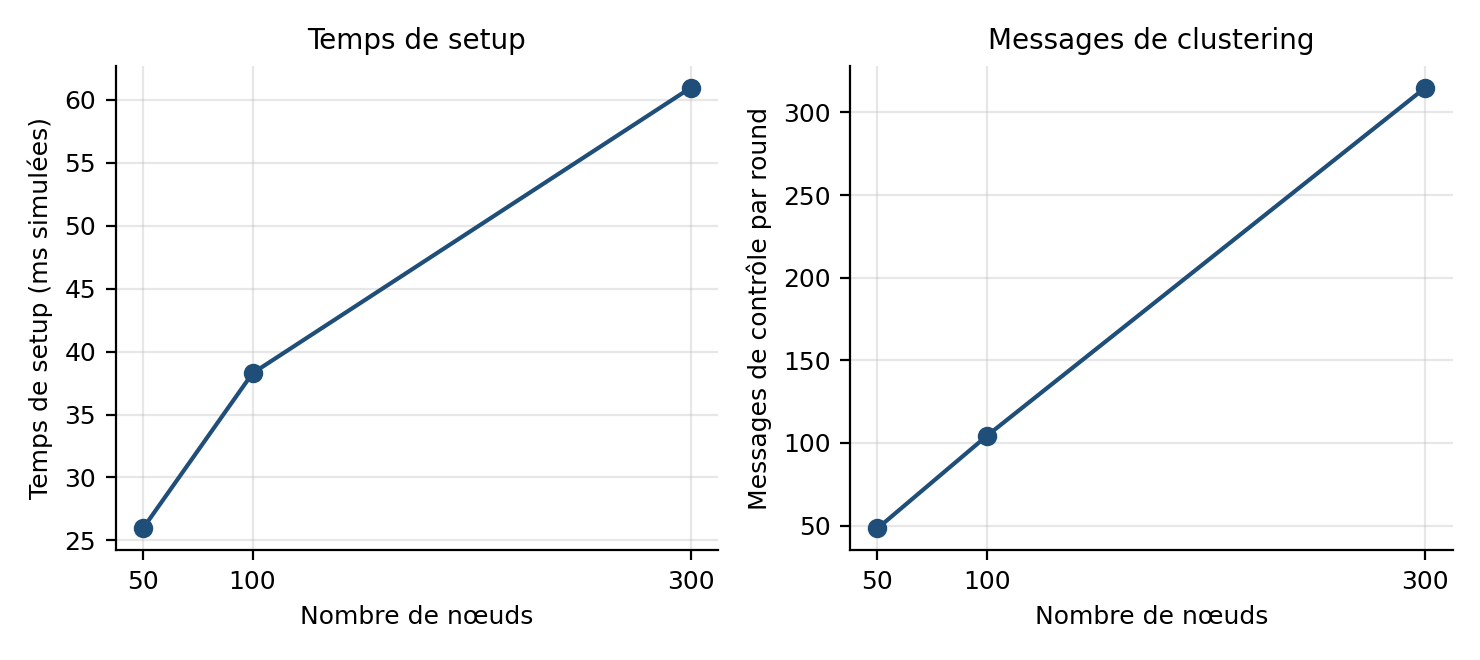
\includegraphics[width=\linewidth]{echelle.png}
\captionof{figure}{Temps de setup (ms simulées) et messages de clustering par round.}\label{fig:echelle}
\end{minipage}

\begin{itemize}
\item \textbf{Messages de clustering.} Ils valent exactement $N+\nCH$ (ADV : $\nCH$ ; JOIN : $N-\nCH$ ; SCHEDULE : $\nCH$), ce que nous avons vérifié sur 100\pct{} des rounds sans nœud mort et avec $\nCH>0$ : la croissance est linéaire en $N$.
À $N=50$ la moyenne (48,2) est inférieure à 52,6 car 8\pct{} des rounds n'ont aucun CH, donc aucun message.
\item \textbf{Temps de setup.} Il passe de 26 à 38 puis 61 ms ($\times2{,}3$ pour $\times6$ nœuds, soit $\propto N^{0{,}48}$). Il vaut (2$\nCH$ + taille du plus gros cluster) $\times$ 0,8 ms (200 bits à 250 kbit/s).
Un cluster garde $\approx1/p=20$ membres, d'où une croissance sous-linéaire ; mais le terme $2\nCH$ (ADV et SCHEDULE séquentiels) pèse 16\pct, 21\pct{} puis 39\pct{} du setup pour $N=50$, 100, 300 et rend la croissance asymptotiquement linéaire.
\item \textbf{FND croissant avec $N$} (99, 191, 271) : à surface fixe, la densité augmente, les clusters sont plus petits et les liaisons membre $\to$ CH plus courtes (consommation initiale 0,40 ; 0,22 ; 0,18\pct{} de l'énergie initiale par round).
Ce n'est pas une amélioration de l'algorithme.
\end{itemize}

\subsection{Expérience C : taux de livraison (paquets de données uniquement)}
\begin{figure}[htbp]
\centering
\begin{subfigure}{0.465\textwidth}\centering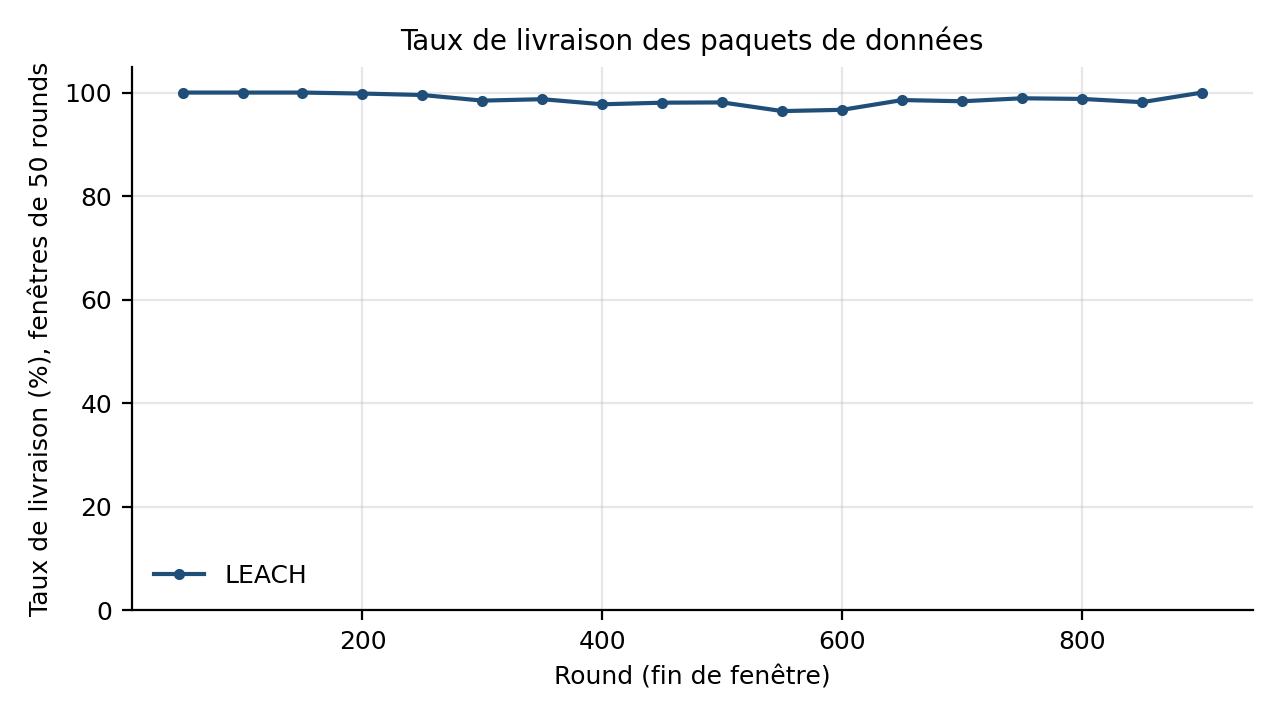
\includegraphics[width=\linewidth]{livraison.png}\caption{Taux de livraison (\%), fenêtres de 50 rounds}\label{fig:liv}\end{subfigure}\hfill
\begin{subfigure}{0.465\textwidth}\centering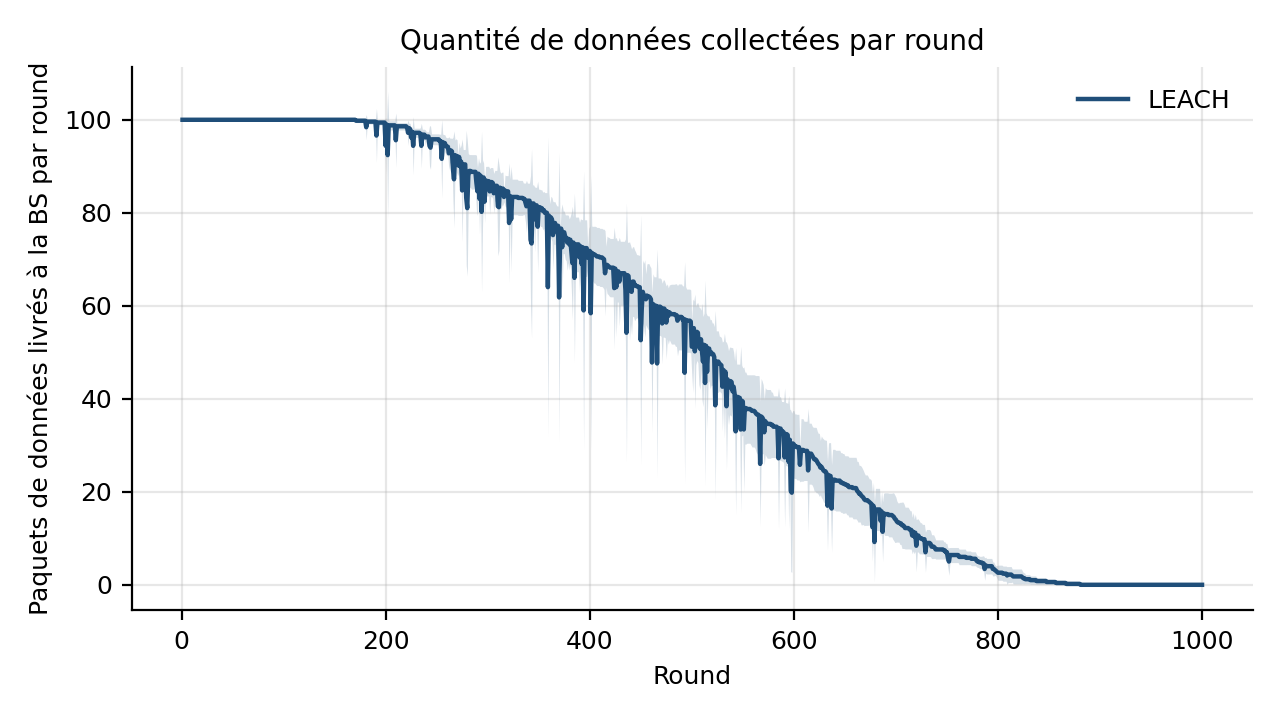
\includegraphics[width=\linewidth]{livraison_par_round.png}\caption{Paquets livrés à la BS par round}\label{fig:livround}\end{subfigure}
\caption{Expérience C : taux de livraison et débit utile ($N=100$, 5 graines).}\label{fig:C}
\end{figure}

Le taux de livraison global est de \textbf{\pmv{98,92}{0,38}\pct} (de 98,16 à 99,17\pct{} selon la graine) : 50\,372 paquets livrés sur 50\,916 émis ; les pertes viennent uniquement des CH qui meurent en plein round.
Avec 2\pct{} de pertes aléatoires il passe à \textbf{\pmv{95,49}{0,36}\pct}, valeur cohérente avec deux sauts successifs ($0{,}98^2\approx96\pct$), et FND/HND/LND restent quasi inchangés (191 / 523 / 840).
Le coût moyen est d'environ 1,0 mJ par paquet livré.

\textbf{Piège d'interprétation.} Le taux reste proche de 100\pct{} alors que le réseau s'effondre, car les nœuds morts n'émettent plus et sortent du dénominateur.
La figure~\ref{fig:livround} montre la réalité : 100 paquets livrés par round au début, $\approx67$ vers le round 425, $\approx10$ vers le round 725 et \textbf{0} sur les 50 derniers rounds. Il faut donc présenter les deux courbes.

% =====================================================================
\section{Critique de NS3}\label{sec:ns3}
\textbf{Facilité d'implémentation.} NS3 ne fournit ni LEACH ni clustering natif, et son cadre d'énergie (\code{EnergySource}, \code{WifiRadioEnergyModel}), calibré sur des radios réelles, ne correspond pas au modèle imposé :
nous avons écrit notre propre comptabilité d'énergie (\code{TxE}/\code{RxE}, une vingtaine de lignes) et la boucle de rounds (\code{Simulator::Schedule}). Points positifs : \code{NodeContainer} et \code{MobilityHelper} (positions), \code{CommandLine} (paramètres sans recompilation),
\code{RngSeedManager::}\allowbreak\code{SetRun} (graines reproductibles), compilation rapide avec trois modules. Points négatifs : courbe d'apprentissage C++ et build
(\code{./ns3 configure/build}, \code{scratch/}), installation lourde sur Mac ARM (VM + compilation), pas d'outil de tracé intégré.

\textbf{Réalisme de la couche radio.} Notre simulation n'utilise ni la couche physique, ni le MAC, ni la propagation de NS3 : pas de collisions ni d'interférences, TDMA parfait, pas d'énergie d'écoute, et un temps de setup calculé
analytiquement (250 kbit/s) et non mesuré ; le taux de livraison ($\approx99\pct$) est donc optimiste. NS3 propose des modèles réalistes (\code{lr-wpan}/IEEE 802.15.4, Wi-Fi, propagation log-distance, collisions) pour envoyer de vrais paquets,
mais l'énergie ne suivrait plus le modèle imposé sans adaptation et il faudrait compiler davantage de modules ($\approx1$ h).

\textbf{Performances et alternatives.} 300 nœuds $\times$ 1000 rounds s'exécutent sans difficulté dans la VM (réglage par défaut du Vagrantfile : 4 Go, 2 vCPU). OMNeT++ (Castalia, INET) apporte des modèles de capteur et de batterie
et une interface graphique, au prix d'un langage supplémentaire (NED) ; TOSSIM exécute le vrai code TinyOS mais s'adapte mal à un modèle d'énergie arbitraire (remarques tirées de leur documentation, non utilisés ici).

% =====================================================================
\section{Comparaison avec DEEC}\label{sec:deec}
Les résultats du binôme DEEC ne sont pas encore disponibles : la colonne DEEC du tableau~\ref{tab:deec} est \textbf{à compléter} (aucune valeur n'est supposée), avec les mêmes paramètres, graines (1 à 5) et format de CSV, puis
\code{plot_results.py --compare "deec_n100_run*.csv" --label DEEC --other-init 60}.

\begin{table}[H]
\centering\small
\begin{tabular}{|l|c|c|p{6.6cm}|}
\hline
\textbf{Métrique ($N=100$)} & \textbf{LEACH (NS3)} & \textbf{DEEC} & \textbf{Attendu}\\ \hline
FND & \pmv{191}{14} & \textit{à compléter} & Nettement plus tardif (élection pondérée par $E_{\text{résiduelle}}/E_{\text{moyenne}}$ [3])\\
HND ; LND & \pmv{519}{29} ; \pmv{844}{31} & \textit{à compléter} & À mesurer\\
Énergie restante au FND & \pmv{58}{4}\pct{} & \textit{à compléter} & CH mieux répartis\\
Livraison globale & \pmv{98,92}{0,38}\pct & \textit{à compléter} & Chute du débit utile plus tardive\\
Messages / round & 104,3 & \textit{à compléter} & Même ordre de grandeur\\ \hline
\end{tabular}
\caption{Comparaison LEACH / DEEC (5 graines).}\label{tab:deec}
\end{table}

Nos résultats motivent déjà cette comparaison : le rapport énergie des CH / énergie moyenne vaut 0,96 (élection sans égard à l'énergie) et la distance à la BS prédit l'ordre de mort. En favorisant les nœuds riches, DEEC devrait retarder le FND.
Pour comparer équitablement, il faudra tenir compte des 20\pct{} de nœuds avancés à 1 J de DEEC (60 J contre 50 J) en traçant l'énergie normalisée : une partie de son avantage viendra de ces nœuds et non du seul algorithme.

% =====================================================================
\section{Conclusion}
Les simulations confirment les limites de LEACH annoncées par le cours.
\begin{enumerate}
\item \textbf{Énergie et durée de vie.} Le premier nœud meurt à 23\pct{} de la durée de vie du réseau (FND 191, LND 844) alors que 58\pct{} de l'énergie reste disponible, parce que l'élection ignore énergie et distance ; le nombre de CH fluctue de 0 à 13.
\item \textbf{Passage à l'échelle.} Les messages valent exactement $N+\nCH$ (linéaire) et le setup est sous-linéaire ($\propto N^{0{,}48}$) : LEACH passe bien à l'échelle côté protocole, mais le FND dépend de la densité.
\item \textbf{Livraison.} Le taux de $\approx99\pct$ est trompeur : le débit utile s'effondre de 100 à 0 paquet par round.
\end{enumerate}
LEACH est donc bien \og un piège \fg{} dans ce scénario où la BS est hors de la zone.

\textbf{Limites.} Canal idéal ; 5 graines seulement ; une seule taille de paquet (la référence Python donne un FND $\approx206$ à 4000 bits, $\approx406$ à 2000 bits et aucun nœud mort en 1000 rounds à 500 bits) ;
unité de $\varepsilon_{\mathrm{mp}}$ à faire valider ; comparaison DEEC à finaliser. \textbf{Perspectives :} intégrer les CSV DEEC, passer à 10 graines, et utiliser de vrais paquets (\code{lr-wpan}) pour obtenir un taux de livraison réaliste.

\begin{thebibliography}{9}\footnotesize\setlength{\itemsep}{0pt}
\item[{[1]}] W. R. Heinzelman, A. Chandrakasan, H. Balakrishnan, \og Energy-efficient communication protocol for wireless microsensor networks \fg, \textit{HICSS}, 2000.
\item[{[2]}] W. R. Heinzelman \textit{et al.}, \og An application-specific protocol architecture for wireless microsensor networks \fg, \textit{IEEE Trans. Wireless Commun.}, 2002.
\item[{[3]}] L. Qing, Q. Zhu, M. Wang, \og Design of a distributed energy-efficient clustering algorithm for heterogeneous wireless sensor networks \fg{} (DEEC), \textit{Computer Communications}, 2006.
\item[{[4]}] Documentation NS3, \texttt{nsnam.org}.
\end{thebibliography}

% =====================================================================
\section*{Annexe}
\begingroup
\VerbatimInput[fontsize=\fontsize{7.2}{8.6}\selectfont,frame=single,framesep=3pt]{../figures/resume.txt}
\endgroup

\end{document}
